\section{Final results}

Since the individual results for each implementation were shown in the respective section, this section shows the global comparative final results.

\Cref{fig:results:final} shows the final speedups obtained for best version of each implementation, compared to the original implementation.

\begin{figure}[!htp]
	\centering
	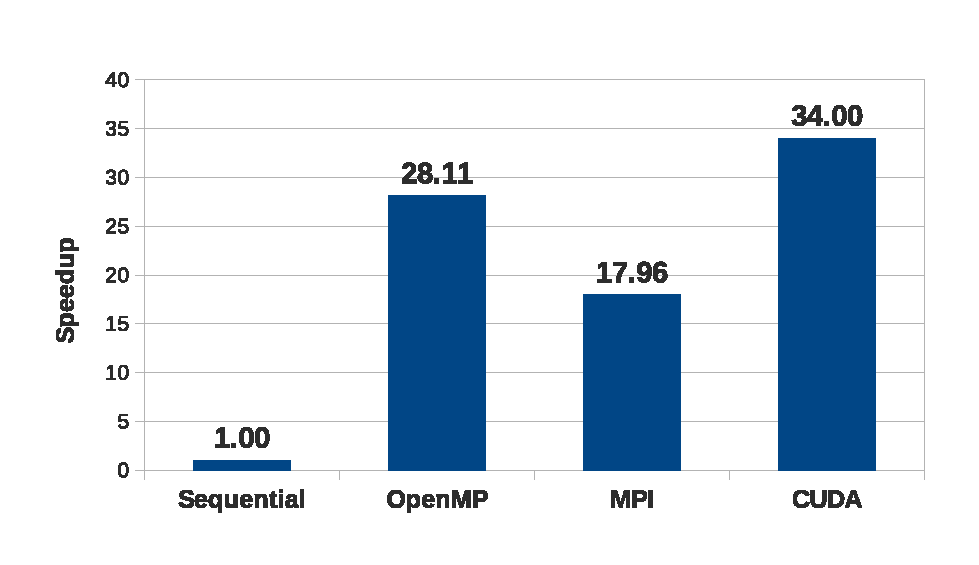
\includegraphics[width=\columnwidth]{images/graph_comparison_all.eps}
	\caption{Speedup results for the best version of each implementation, compared with the original implementation.}
	\label{fig:results:final}
\end{figure}

The best results were clearly obtained with the massively parallel implementation using CUDA. Yet, the shared memory version achieved a very similar value, specially taking into account that it could benefit from the latest most significant optimization performed in the CUDA implementation.
Yet, this happens probably to the lack of a test case big enough to take advantage of all the hardware resources in the GPU, which was not possible to generate.

The distributed memory implementation achieved a speedup which is nearly half the other two versions.
While this implementation was not target of so many optimizations as the other two versions, it faces the same locality problems (although these are softened because the mesh is now divided among the computational nodes) and adds the comunication overhead.
This overhead easily becomes the bottleneck of this implementation, specially when using many computational nodes with only a few processors.
